\PassOptionsToPackage{dvipsnames}{color}
\PassOptionsToPackage{dvipsnames}{xcolor}
% >>> j2l compat: xcolor / named-colour compatibility
\PassOptionsToPackage{dvipsnames}{color}
\PassOptionsToPackage{dvipsnames,svgnames,x11names,table}{xcolor}
\RequirePackage{xcolor}
\makeatletter\@namedef{ver@color.sty}{2021/01/01}\makeatother
\makeatletter\@ifundefined{providecolor}{}{%
  \providecolor{Bittersweet}{RGB}{128,128,128}
  \providecolor{Dandelion}{RGB}{128,128,128}
  \providecolor{abstractcolor}{RGB}{128,128,128}
  \providecolor{rulecolor}{RGB}{128,128,128}
}\makeatother
% <<< j2l compat
\documentclass[10pt]{NSP1}
\IfFileExists{url.sty}{\usepackage{url}}{}
\IfFileExists{floatflt.sty}{\usepackage{floatflt}}{}
\IfFileExists{helvet.sty}{\usepackage{helvet}}{}
\IfFileExists{times.sty}{\usepackage{times}}{}
\IfFileExists{psfig.sty}{\usepackage{psfig}}{}
\IfFileExists{graphics.sty}{\usepackage{graphics}}{}
\IfFileExists{mathptmx.sty}{\usepackage{mathptmx}}{}
\IfFileExists{amsmath.sty}{\usepackage{amsmath}}{}
\IfFileExists{amssymb.sty}{\usepackage{amssymb}}{}
\IfFileExists{bm.sty}{\usepackage{bm}}{}
\IfFileExists{float.sty}{\usepackage{float}}{}
\IfFileExists{caption.sty}{\usepackage[bf,hypcap]{caption}}{}
%% --- additional packages required by the tables and figures of this paper ---
\IfFileExists{graphicx.sty}{\usepackage{graphicx}}{}
\IfFileExists{longtable.sty}{\usepackage{longtable}}{}
\IfFileExists{booktabs.sty}{\usepackage{booktabs}}{\providecommand\toprule{\hline}\providecommand\midrule{\hline}\providecommand\bottomrule{\hline}}
\IfFileExists{array.sty}{\usepackage{array}}{}
\IfFileExists{calc.sty}{\usepackage{calc}}{}
\IfFileExists{multirow.sty}{\usepackage{multirow}}{\providecommand\multirow[3]{#3}}

\providecommand{\tightlist}{\setlength{\itemsep}{0pt}\setlength{\parskip}{0pt}}
\providecommand{\real}[1]{#1}
\providecommand{\ul}[1]{\underline{#1}}
\providecommand{\hl}[1]{#1}
\providecommand{\RL}[1]{#1}
\providecommand{\textquotesingle}{'}
\DeclareUnicodeCharacter{03B1}{$\alpha$}
\DeclareUnicodeCharacter{03B2}{$\beta$}
\DeclareUnicodeCharacter{03C7}{$\chi$}
\DeclareUnicodeCharacter{03C1}{$\rho$}
\DeclareUnicodeCharacter{03BC}{$\mu$}
\DeclareUnicodeCharacter{03C3}{$\sigma$}
\DeclareUnicodeCharacter{2264}{$\leq$}
\DeclareUnicodeCharacter{2265}{$\geq$}
\DeclareUnicodeCharacter{2260}{$\neq$}
\DeclareUnicodeCharacter{00D7}{$\times$}
\DeclareUnicodeCharacter{00B1}{$\pm$}
\DeclareUnicodeCharacter{2248}{$\approx$}
\DeclareUnicodeCharacter{221A}{$\sqrt{\ }$}
\DeclareUnicodeCharacter{2192}{$\rightarrow$}
\DeclareUnicodeCharacter{2022}{$\bullet$}
\DeclareUnicodeCharacter{00B7}{$\cdot$}
\DeclareUnicodeCharacter{2032}{$'$}
\DeclareUnicodeCharacter{0393}{$\Gamma$}
\DeclareUnicodeCharacter{03B7}{$\eta$}
\DeclareUnicodeCharacter{03B8}{$\theta$}
\DeclareUnicodeCharacter{03BB}{$\lambda$}
\DeclareUnicodeCharacter{03A3}{$\Sigma$}
\DeclareUnicodeCharacter{03B4}{$\delta$}
\DeclareUnicodeCharacter{03B3}{$\gamma$}
\DeclareUnicodeCharacter{2026}{\ldots}
\DeclareUnicodeCharacter{FEFF}{}

\tolerance=1
\emergencystretch=\maxdimen
\hyphenpenalty=10000
\hbadness=10000

\topmargin=0.00cm

\def\sm{\smallskip}
\def\no{\noindent}

\def\firstpage{1}
\setcounter{page}{\firstpage}
\def\thevol{No}
\def\thenumber{}
\def\theyear{}

\IfFileExists{graphicx.sty}{\usepackage{graphicx}}{}
\makeatletter
\def\biographyps#1#2{%
  \par\addvspace{21dd}\small\noindent
  \if!#1!\else
    \noindent\includegraphics[width=1in,height=1.25in,keepaspectratio]{#1}\par\smallskip
  \fi
  {\bfseries#2\unskip\ }\ignorespaces}
\def\endbiographyps{\par\addvspace{12pt}}
\makeatother
\IfFileExists{xcolor.sty}{\usepackage[table]{xcolor}}{}
\IfFileExists{array.sty}{\usepackage{array}}{}
\IfFileExists{cuted.sty}{\usepackage{cuted}}{\newenvironment{strip}{\par\medskip\noindent\begin{minipage}{\linewidth}}{\end{minipage}\par\medskip}}
\makeatletter
\newcommand\jltx@wideopen{\par\addvspace{\medskipamount}\noindent}
\newcommand\jltx@wideclose{\par\addvspace{\medskipamount}}
\newenvironment{jltxspan}
  {\if@twocolumn\let\jltx@spannext\strip\else\let\jltx@spannext\jltx@wideopen\fi\jltx@spannext}
  {\if@twocolumn\let\jltx@spanend\endstrip\else\let\jltx@spanend\jltx@wideclose\fi\jltx@spanend}
\makeatother
\newcommand\JLTXaboveplacement{\par\addvspace{6pt plus 2pt minus 2pt}\noindent}
\newcommand\JLTXbelowplacement{\par\addvspace{6pt plus 2pt minus 2pt}}
\widowpenalty=10000
\clubpenalty=10000
\IfFileExists{newunicodechar.sty}{\usepackage{newunicodechar}}{\makeatletter\providecommand\newunicodechar[2]{%
  \begingroup\lccode`\~=`#1\lowercase{\endgroup\def~}{#2}%
  \catcode`#1=\active}\makeatother}
\newunicodechar{α}{\ensuremath{\alpha}}
\newunicodechar{≤}{\ensuremath{\leq}}

% >>> j2l compat: scalable Computer Modern (arbitrary font sizes)
\IfFileExists{type1cm.sty}{\usepackage{type1cm}}{}
\IfFileExists{fix-cm.sty}{\usepackage{fix-cm}}{}
% <<< j2l compat
\begin{document}
% >>> j2l compat: body-text size (+5%)
\makeatletter
\edef\JLTXbasesize{\f@size}
\@tempdimb=1.2\dimexpr\f@size pt\relax\edef\JLTXbaseskip{\strip@pt\@tempdimb}
\def\JLTXbodyscale{1.050}
\let\JLTX@normalsize\normalsize
\renewcommand\normalsize{%
  \JLTX@normalsize
  \@tempdima=\JLTXbodyscale\dimexpr\f@size pt\relax
  \@tempdimb=1.2\@tempdima
  \fontsize{\strip@pt\@tempdima}{\strip@pt\@tempdimb}\selectfont}%
\@ifundefined{@makecaption}{}{%
  \let\JLTX@makecaption\@makecaption
  \long\def\@makecaption#1#2{%
    \begingroup\fontsize{\JLTXbasesize}{\JLTXbaseskip}\selectfont
    \let\normalsize\JLTX@normalsize
    \JLTX@makecaption{#1}{#2}\endgroup}}%
\@ifundefined{thebibliography}{}{%
  \let\JLTX@thebibliography\thebibliography
  \def\thebibliography{%
    \fontsize{\JLTXbasesize}{\JLTXbaseskip}\selectfont\JLTX@thebibliography}}%
\makeatother
\normalsize
% <<< j2l compat

% >>> j2l: keep the journal banner with the title block
\makeatletter
\let\JLTXorig@newpage\newpage
\let\JLTXorig@clearpage\clearpage
\let\JLTXorig@cleardoublepage\cleardoublepage
\let\newpage\relax\let\clearpage\relax\let\cleardoublepage\relax
\makeatother
% <<< j2l


\titlefigurecaption{{\large \bf \rm Journal of Statistics Applications \& Probability }\\ {\it\small An International Journal}}

\title{Psychological factors influencing administrative decision-making among educational leaders: A cognitive psychology perspective}

\author{Dr. Falah Dhuwaihi Al-Swairi Al-Ajmi$^{1}$}
\institute{$^{1}$ Department of Educational Foundations and Administration/Faculty of Educational Sciences, Amman Arab University, -Jordan, , : 0009-000804609-0140}

\titlerunning{Psychological factors influencing administrative decision-making among educational leaders: A cognitive psychology perspective}
\authorrunning{Dr. Falah Dhuwaihi Al-Swairi Al-Ajmi}

%corresponding author email
\mail{f.dhuwaihi@aau.edu.jo}

\received{7 June. 2026}
\revised{20 June. 2026}
\accepted{22 July 2026.}
\published{0 -8-2026.}

\abstracttext{This study looked at the psychological factors that shape the way educational leaders take administrative decisions, and read them from the side of cognitive psychology. It aimed to find the cognitive and psychological factors most common among leaders when they reach a decision, to look at the link between some cognitive biases and the quality of those decisions, and to compare analytical thinking with rapid thinking inside the educational setting. The study followed the descriptive approach and used the Delphi technique, where a chosen panel of thirty educational experts answered an electronic questionnaire built on a five-point scale and drawn from the theoretical literature. The answers were summed up by descriptive statistics, and the links were read by a rank-order correlation together with a paired comparison of the two thinking styles. Confidence intervals and effect sizes were worked out to help the reading. The study found that cognitive and psychological factors have a large share in the way educational leaders reach their decisions. Analytical, ordered thinking came first, then rapid intuitive thinking, while tolerance for ambiguity came last. Each bias that was looked at went with a lower quality of decision, and the strongest link was for loss aversion, then confirmation bias, then the framing effect. The comparison of the two styles showed that analytical thinking went with a clearly higher effectiveness than rapid thinking. On this base, the study recommends putting the ideas of cognitive psychology inside the preparation and the professional development of educational leaders, so that they become aware of their own thinking patterns and of how far a bias can reach them, and building programmers that strengthen analytical reasoning and decision-making that stands on evidence. The study adds a cognitive and psychological reading of administrative decision-making beside the organizational and procedural readings that fill the regional literature, and gives a base for later work that ties personal and professional variables to the decision behaviour of leaders.}

\keywords{Psychological factors, administrative decision-making, cognitive psychology}

\maketitle
% >>> j2l: page breaking restored after the title block
\makeatletter
\let\newpage\JLTXorig@newpage
\let\clearpage\JLTXorig@clearpage
\let\cleardoublepage\JLTXorig@cleardoublepage
\makeatother
% <<< j2l


\raggedbottom
\setlength{\textfloatsep}{12pt plus 2pt minus 2pt}
\setlength{\intextsep}{12pt plus 2pt minus 2pt}
\setlength{\floatsep}{12pt plus 2pt minus 2pt}


\par\vspace{6.0pt}\noindent {\normalsize 1 Introduction:\par}\vspace{12.0pt}

Decision-making is a key driver of the effectiveness of organizations of all types. It is linked to the ability to direct, manage resources, and achieve goals in complex and rapidly changing environments.

This process is also influenced by the nature of the organizational context, the pressures of reality, and the individual characteristics of the decision-maker. This makes administrative decisions the product of the interaction of multiple factors, some of which are overt, related to regulations and structures, and others latent, connected to the mental and psychological processes that govern thinking, evaluation, and selection [1].

Educational institutions acquire a double dimension due to the direct connection of their decisions to human destinies and to long-term educational, ethical, and developmental dimensions. Educational leaders operate in an environment where academic, organizational, and social considerations intersect, where levels of uncertainty are increasing, and where they are subject to frequent time and professional pressures. This makes their decisions susceptible to being influenced by their prevailing thinking patterns, their methods of processing information, and their responses to emergencies or routine situations [2].

Contemporary trends in psychological and administrative studies indicate that administrative decisions are not always based on purely rational analysis. Rather, they are often shaped by unconscious cognitive processes, biases, and rapid or analytical thinking patterns, the intensity of which varies depending on the situation, experience, and environment. This explains the noticeable variation in the quality of administrative decisions, even among leaders with similar qualifications and organizational circumstances [3].

Despite the growing interest in the topic of educational leadership and administrative decision-making, the cognitive-psychological factors aspect still has a limited presence in Arab studies, as the focus is mostly on organizational or procedural dimensions, while neglecting the role that the leader's internal mental processes play in guiding his choices and interpreting alternatives [4]. This limits the comprehensive understanding of the nature of administrative decision-making in the educational environment. Based on this, this study comes to highlight the cognitive-psychological factors affecting administrative decision-making among educational leaders from the perspective of cognitive psychology, seeking to identify the most prominent of these factors, analyze the nature of their impact on the quality and efficiency of the decision, and reveal the differences related to some professional and demographic variables, in order to contribute to building a deeper scientific understanding of the decision-making process and support efforts aimed at rationalizing leadership practices in educational institutions.

Problem Statement:

The decision-making process is a cornerstone of effective leadership within educational institutions. It is linked to the educational leader's ability to guide institutional work, organize resources, and respond to the demands of the changing educational environment. This process involves multiple organizational and professional factors, along with mental and cognitive processes that govern understanding situations, evaluating alternatives, and selecting the most suitable option. This makes administrative decision-making a complex process that transcends apparent procedural aspects. Often, the interpretation of administrative decisions issued by educational leaders is reduced to organizational frameworks or professional experiences, without delving into the analysis of the cognitive and psychological factors that influence the decision-making process itself. This limits our ability to understand the reasons for the variation in the quality and efficiency of administrative decisions within educational institutions [5].

Hence the need to study these factors from a cognitive psychology perspective. Thus, the problem of this study can be summarized in the following main question: What cognitive and psychological factors influence administrative decision-making among educational leaders from a cognitive psychology perspective? This leads to the following sub-questions:

\begin{enumerate}
  \item What are the most prominent cognitive and psychological factors prevalent among educational leaders when making their administrative decisions?
  \item What is the nature of the relationship between cognitive biases (confirmation bias, framing effect, loss aversion) and the quality and effectiveness of administrative decisions made by educational leaders?
  \item To what extent does the thinking style (fast-tracking versus analytical) affect the effectiveness of administrative decisions made by educational leaders in different administrative situations?
\end{enumerate}

Study Objectives:

This study aims to achieve the following objectives:

\begin{enumerate}
  \item To identify the most prominent cognitive and psychological factors prevalent among educational leaders when making their administrative decisions.
  \item To analyze the nature of the relationship between cognitive biases (confirmation bias, framing effect, loss aversion) and the quality and efficiency of administrative decisions made by educational leaders.
  \item To reveal the impact of thinking style (rapid thinking versus analytical thinking) on ​​the effectiveness of administrative decision-making among educational leaders in different administrative situations.
\end{enumerate}

Significance of the Study:

First: Theoretical Significance:

The theoretical significance of this study stems from its aim to deepen the scientific understanding of the cognitive-psychological factors influencing administrative decision-making among educational leaders. This is achieved by employing concepts and models from cognitive psychology, particularly dual reasoning theory and cognitive bias theory, within the field of educational leadership. The study contributes to enriching the Arabic literature in this area by:

\begin{enumerate}
  \item Providing an explanatory framework that links the internal cognitive processes of the educational leader to their behaviors in administrative decision-making.
  \item Uncovering cognitive-psychological dimensions that are often neglected in traditional administrative studies, which focus on organizational and procedural aspects.
  \item Filling a research gap represented by the scarcity of studies that have addressed administrative decision-making in educational institutions from a cognitive-psychological perspective.
  \item Providing a theoretical foundation upon which future studies can be built, addressing other cognitive and psychological variables related to educational leadership.
\end{enumerate}

Second: Practical Significance:

The practical significance of this study lies in the potential for utilizing its findings to improve administrative decision-making practices in educational institutions, through:

\begin{enumerate}
  \item Helping educational leaders become aware of cognitive biases that may negatively affect their administrative decisions.
  \item Contributing to the design of training and professional development programs aimed at developing analytical thinking skills and reducing excessive reliance on intuitive thinking in sensitive situations.
  \item Supporting educational policymakers in adopting more rational and flexible decision-making models that consider the psychological and cognitive aspects of leaders.
  \item Improving the quality and efficiency of administrative decisions, which will positively impact institutional performance, organizational stability, and the quality of the educational process.
\end{enumerate}

Theoretical Framework of the Study:

First: Administrative Decision-Making in Educational Institutions:

\par\medskip\noindent {\normalsize\bfseries 1. The Nature of Administrative Decision-Making in the Educational Context:\par}\smallskip

Administrative decision-making in educational institutions is a central process that takes shape within a dynamic learning environment. Educational, organizational, and social considerations intertwine, and the decision is influenced by time constraints, available resources, and stakeholder demands [6]. Decision-making acquires a unique character that distinguishes the educational environment from other sectors. It requires the educational leader to balance short-term and long-term goals, ensure effective implementation, and address unforeseen situations in a way that guarantees the continuity of the educational process and the quality of its outcomes [7].

The decision-making process relies on a continuous interaction between experience, knowledge, and cognitive analysis [8]. The leader evaluates available alternatives, utilizes intuition and experience when necessary, and deals wisely with incomplete information. This also includes interaction with teachers, students, and stakeholders, and consideration of the institution's cultural and organizational context [9], [10]. The researcher emphasizes that the leader's understanding of human nature within the institution enhances the quality of the decision and reduces deviation from educational objectives [14].

\par\medskip\noindent {\normalsize\bfseries 2. Levels and Types of Educational Administrative Decisions:\par}\smallskip

Administrative decisions in educational institutions are distributed across multiple levels. Their impact and processing methods vary according to the nature of each level. These include operational decisions, which deal with daily activities such as scheduling classes and monitoring performance. These are characterized by rapid implementation and the need for the leader's intuition and experience [11]. Organizational decisions relate to resource allocation, regulating internal relationships, and defining specific policies. These require gathering accurate information and comparing alternatives to minimize risks. Strategic decisions, which involve guiding the institution in the long term, such as adopting new educational programs or development plans, necessitate in-depth analysis and a study of the consequences of each alternative before making a decision [12].

The researcher indicates that a leader's awareness of the decision level helps them choose the appropriate thinking style. He emphasizes that confusing the levels leads to weakened decision effectiveness and disruption of workflow. Distinguishing between the levels is highlighted as a tool to enhance the leader's ability to utilize their skills and experience accurately and effectively.

\par\medskip\noindent {\normalsize\bfseries 3.The Role of the Educational Leader in Guiding Administrative Decision-Making:\par}\smallskip

The educational leader plays a pivotal role in guiding the decision-making process within educational institutions. They interpret situations, assess alternatives, and manage risks. Their decisions are a comprehensive response to the pressures of the institution and the needs of the community, and their leadership style reflects the institution's ability to adapt to challenges and changes [13].

The leader relies on their professional experience to understand the educational environment and analyze information. They benefit from interaction with teachers, students, and stakeholders to evaluate situations and balance intuition and logical analysis when processing incomplete information. Their decisions are influenced by professional and personal values ​​that determine their approach to risk assessment and alternative selection [14].

The researcher points out that the leader is not merely an implementer of regulations and instructions, but a cognitive agent who shapes decisions according to their cognitive framework and acquired experiences. The researcher also emphasizes that the cognitive leader's role is not limited to the administrative aspect, but includes guiding the institution towards achieving its strategic goals while considering the human and contextual variables that affect the decision-making process.

Second: Cognitive Psychology and its Relationship to Decision-Making:

\par\medskip\noindent {\normalsize\bfseries 1.The Role of Mental Processes in Understanding Information and Making Decisions:\par}\smallskip

In cognitive psychology, core mental processes are considered one of the fundamental factors that determine how a leader processes information. Administrative decisions are formed in an environment characterized by ambiguity and complexity, necessitating the ability to interpret data, draws conclusions, and connects information to real-world situations. This interaction between knowledge and experience reflects the leader's response to emerging changes within the educational institution [15].

Leaders deal with information using a combination of intuition and logical analysis. They rely on their past experiences to evaluate alternatives and balance speed and accuracy. This includes the ability to recognize recurring patterns and predict the potential consequences of each choice. The impact of these processes is evident in improving the quality of decisions and reducing errors that may result from superficial or overly rapid processing [16, 17]

The researcher points out that a leader's awareness of how they process information enhances their decision-making flexibility and ability to adapt to changing circumstances without compromising desired outcomes. Furthermore, mental processes are not merely intellectual tools, but rather a force that guides managerial behavior and determines the effectiveness of decisions within a complex educational context.

\par\medskip\noindent {\normalsize\bfseries 2. Rapid Thinking vs. Analytical Thinking:\par}\smallskip

The thinking style employed by a leader is one of the most prominent determinants of the nature of managerial decisions. Two main types of processing can be distinguished: rapid or intuitive thinking, which relies on immediate responses to data, and analytical or slow thinking, which depends on systematic study and comparison of alternatives. The choice between these two styles usually arises according to the nature of the situation. Routine decisions require speed of execution, while strategic decisions necessitate in-depth analysis. Leaders rely on intuitive thinking in urgent or time-sensitive situations, where experience and spontaneity allow for a rapid response. Analytical thinking, on the other hand, guides the leader toward carefully studying alternatives, enabling the identification of expected outcomes and planning to mitigate risks [18].

The researcher points out that a balance between these two patterns contributes to improved decision quality and reduces reliance on cognitive biases that can arise from overusing one pattern at the expense of the other [19]. He highlights the importance of developing a leader's skills in switching between fast and slow thinking, adapting to the nature of each situation. Furthermore, a leader's awareness of the cognitive patterns they use in processing information contributes to more accurate and flexible decision-making and forms the basis for minimizing cognitive errors.

\par\medskip\noindent {\normalsize\bfseries 3. Cognitive Biases and Their Impact on Decision-Making:\par}\smallskip

Cognitive biases play a pivotal role in guiding leaders' decisions. These biases represent a tendency to interpret or evaluate based on past experiences or specific mental preconceptions. They manifest in various forms, such as the inclination to seek information that confirms existing beliefs, being influenced by how a problem is presented, or avoiding losses even at the expense of potential gains. This influence makes decisions more prone to error if the leader is unaware of these cognitive tendencies. Managerial decisions are affected by biases to varying degrees depending on experience, the nature of the decision, time constraints, and the leader's ability to verify and analyze information objectively. Understanding these biases and enabling leaders to recognize them allows them to adjust their approach to situations and improve the quality of their decisions. It also helps in developing management training methods that promote critical thinking and reduce the impact of undesirable biases [20, 21].

It becomes clear to the researcher that cognitive biases are an element that cannot be ignored in the study of administrative decision-making, and that the leader’s awareness of these biases enhances his ability to make more balanced and effective decisions in the educational context.

Third: Psychological and Cognitive Factors Affecting Administrative Decision-Making:

\par\medskip\noindent {\normalsize\bfseries 1. Thinking Styles and Their Impact on Decision-Making:\par}\smallskip

Thinking style plays a pivotal role in guiding the decision-making process for educational leaders. It determines how information is processed and available alternatives are assessed. Its impact is clearly evident when comparing routine decisions requiring rapid response with strategic decisions that necessitate in-depth study and careful analysis. A leader's understanding of this process enables them to choose the most appropriate approach for each situation, taking into account the nature and complexity of the decision [22].

Leaders rely on intuitive thinking in urgent or time-sensitive situations, where experience and spontaneous responses allow them to process information quickly. In contrast, analytical thinking guides leaders toward carefully studying alternatives and enables accurate evaluation of potential outcomes [23].

The researcher emphasizes that balancing intuition and analysis contributes to improving decision quality and reducing errors resulting from over-reliance on one style at the expense of the other. He highlights the importance of developing a leader's skills in shifting between different thinking styles to suit each situation and ensure optimal outcomes. Furthermore, understanding a leader's thinking styles is a fundamental approach to analyzing and enhancing the efficiency of the decision-making process [24].

\par\medskip\noindent {\normalsize\bfseries 2. Tolerance for Ambiguity and Psychological Pressure:\par}\smallskip

Decision-making in educational institutions requires a high capacity to cope with ambiguity and psychological pressure. Leaders often encounter situations with incomplete information and need to assess risks and potential outcomes. This reflects adaptability and flexibility in decision-making. A leader with a greater tolerance for ambiguity is more effective in uncertain circumstances, while a lower tolerance leads to hesitation or conservative decisions that reduce the institution's efficiency. A leader's ability to tolerate ambiguity interacts with the pressures arising from direct responsibility for educational outcomes and the need to balance the demands of teachers, students, and stakeholders [25].

The researcher indicates that training leaders to handle complex situations and developmental adaptability enhances decision quality, reduces the impact of psychological stress, and promotes critical thinking and decision-making in uncertain circumstances. The researcher also finds that tolerance for ambiguity and psychological pressure are key factors determining the effectiveness of administrative decisions in educational institutions.

\par\medskip\noindent {\normalsize\bfseries 3. Cognitive Biases and Their Impact on Decision Quality:\par}\smallskip

Cognitive biases are among the most important psychological factors affecting administrative decision-making. They influence the interpretation of information, the evaluation of alternatives, and the final choice. This manifests in the tendency to seek information that confirms pre-existing beliefs, being influenced by how a problem is presented, or being averse to loss at the expense of potential gains. This influence makes decisions more prone to errors if the leader is unaware of these cognitive tendencies [26, 27].

The impact of biases varies depending on the leader's experience, the nature of the decision, time constraints, and their ability to process information objectively. Recognizing biases and empowering leaders to be aware of them allows them to modify their information processing methods and improve the quality of their decisions. It also contributes to designing training programs that enhance critical thinking and reduce the impact of negative biases. It is clear that biases cannot be completely eliminated, but they become manageable when they are recognized and cognitive processes are strategically utilized [28].

The researcher finds that cognitive biases are a fundamental factor in administrative decision-making, and that awareness of them enhances a leader's ability to make balanced and effective decisions within the educational context.

\par\medskip\noindent {\normalsize\bfseries 4. Integrating Psychocognitive Factors with Professional Experience:\par}\smallskip

The integration of cognitive factors with a leader's professional experience is a crucial factor in the effectiveness of administrative decisions. Acquired experience transforms into a cognitive framework through which information can be interpreted, more accurate decisions made, and errors resulting from relying on intuition or biases reduced. This integration enhances the ability to adapt to complex and changing situations within the educational institution [25].

Professional experience supports cognitive processing, enabling leaders to anticipate the potential consequences of each decision, facilitate the handling of incomplete information, and develop self-assessment and evaluation skills. Furthermore, investing in developing a leader's practical experience amplifies the impact of positive psychological factors and mitigates the effects of biases and psychological pressures, thus forming a foundation for improving the quality of administrative decisions and enhancing institutional performance [24].

The researcher concludes that integrating cognitive psychological factors with professional experience represents an effective strategy for enhancing the quality of administrative decisions and achieving the educational institution's goals effectively and flexibly.

Fourth: Models and Theories Explaining Decision-Making from a Cognitive Perspective:

\par\medskip\noindent {\normalsize\bfseries 1. Dual Thinking Theory and its Role in Decision Analysis:\par}\smallskip

Dual thinking theory is considered one of the most prominent models explaining how leaders make decisions from a cognitive perspective. It distinguishes between two thinking systems: the fast, intuitive system, which relies on automatic responses to situations, and the slow, analytical system, which relies on systematic processing and careful consideration of alternatives. The impact of these systems is clearly evident in routine decisions versus strategic decisions. Understanding this theory allows leaders to recognize situations where they rely on intuition or analysis and to choose the most appropriate approach based on the nature of the decision [29].

In emergency situations, a leader relies on the fast system, where their experience and automatic response allow them to process information quickly and effectively. Conversely, they use the slow system when making strategic decisions that require studying the long-term consequences of each alternative. A balance between the two systems contributes to enhancing decision quality and reducing cognitive errors. Management training plays a crucial role in enabling leaders to switch between the two systems as needed. The impact of this theory is evident in improving flexibility and adaptability to diverse challenges within educational institutions [15].

The researcher believes that understanding this theory helps leaders consciously utilize their cognitive processes, thereby enhancing the quality of their decisions and making them more relevant to real-world circumstances.

\par\medskip\noindent {\normalsize\bfseries 2. Cognitive Bias Theory and Its Impact on Decision-Making:\par}\smallskip

Cognitive bias theory provides an important framework for understanding the challenges leaders face when making decisions. It describes how cognitive tendencies influence the interpretation of information and the evaluation of alternatives. This manifests in leaders' tendency to seek information that confirms pre-existing beliefs, to be influenced by how a problem is presented, or to experience a fear of loss. A lack of awareness of these biases leads to less effective and more error-prone decisions, while awareness can modify information processing methods and improve outcomes [12].

Recognizing biases affects the level of expertise, the nature of the decision, and surrounding pressures. It enables leaders to use rational methods to balance intuition and analysis. Furthermore, it contributes to the development of training programs aimed at enhancing critical thinking and reducing the negative impact of biases [13].

The researcher points out those biases cannot be completely eliminated, but they become manageable when leaders are aware of their tendencies and strategically utilize mental processes to achieve more accurate and objective decisions.

\par\medskip\noindent {\normalsize\bfseries 3. Integrating Theories and Cognitive Processes in Leadership Practice:\par}\smallskip

Leaders can benefit from integrating theoretical models with practical experience in managing educational institutions. Understanding dual thinking and cognitive biases becomes a tool for guiding the mental processing of information, analyzing alternatives, and making more conscious decisions. This integration allows for the identification of strengths and weaknesses in decision-making styles and improves overall administrative performance [30], [31].

Leaders rely on this knowledge to evaluate routine and strategic decisions more effectively. It also enables them to guide their teams, reduce the impact of biases, and increase their ability to handle stress and unexpected situations. Furthermore, the integration of theory and experience enhances adaptability and flexibility, aligns decisions more closely with the goals of the educational institution, and increases the effectiveness of cognitive leadership [32].

The researcher emphasizes that integrating theories and cognitive processes provides a robust framework for understanding educational administrative decisions and contributes to enhancing the quality and efficiency of decisions, leading to more effective and sustainable achievement of the institution's goals.

Third: Study Methodology and Tools:

\par\medskip\noindent {\normalsize\bfseries 1.Study Methodology:\par}\smallskip

Ethical Considerations

This study adhered to established ethical standards for research involving human participants. Participation was voluntary, and informed consent was obtained from all participants prior to their involvement in the study. Confidentiality and anonymity were ensured, and participants were informed of their right to withdraw at any time without any consequences.

As the affiliated institution does not have a formal Institutional Review Board (IRB), formal ethical approval was not required. However, the study followed recognized international ethical guidelines for research involving human participants.

For transparency, the study aligns with the ethical principles outlined by the World Medical Association Declaration of Helsinki:

https://www.wma.net/what-we-do/medical-ethics/declaration-of-helsinki.

All procedures performed in this study were conducted in accordance with ethical standards of educational research and institutional guidelines.

Informed Consent

Verbal informed consent was obtained from all participants prior to data collection. Written consent was not required due to the nature of the study, which posed minimal risk and did not involve sensitive personal data.

Verbal consent was considered appropriate in this context to facilitate participation and reduce administrative burden, particularly within the educational setting.

Participants were clearly informed about the purpose of the study, their right to withdraw at any time, and the confidentiality of their responses.

The consent process was documented by the researcher through confirmation records, and all data were securely stored in compliance with data protection and research ethics standards.

\par\medskip\noindent {\normalsize\bfseries 2. Study Population:\par}\smallskip

The study population consisted of experts and educational leaders working in educational institutions that possess professional experience in the administrative and educational fields and participate in or supervise administrative decisions. This is because they are capable of providing accurate assessments of the nature of the cognitive and psychological processes accompanying decision-making in the educational context.

\par\medskip\noindent {\normalsize\bfseries 3. Study Sample:\par}\smallskip

A purposive sample of (30) educational experts was selected according to specific criteria, including extensive professional experience in educational and administrative work, active participation in leadership or supervisory positions, and a willingness to contribute scientifically to the study. This sample size is suitable for the Delphi methodology, which does not aim for statistical generalization but rather seeks to deepen understanding through specialized, high-quality expertise.

\par\medskip\noindent {\normalsize\bfseries 4. Study Instrument:\par}\smallskip

The study employed an electronic questionnaire designed based on the theoretical framework and previous studies. It consisted of three main sections, the first section addressed the prevailing cognitive and psychological factors among educational leaders, the second section focused on cognitive biases and their relationship to the quality and efficiency of administrative decisions. The third section examined thinking patterns and their impact on the effectiveness of administrative decisions, the questionnaire items were formulated using a five-point Likert scale to ensure measurement accuracy and ease of statistical analysis.

\par\medskip\noindent {\normalsize\bfseries 5. Instrument Validity and Reliability:\par}\smallskip

The instrument's validity was established by presenting it to a panel of expert reviewers specializing in educational administration and educational psychology. This ensured the suitability of the items to the study's objectives, the clarity of their wording, and their comprehensiveness across the research areas. Their feedback was taken into account, and the necessary modifications were made, contributing to the enhancement of both the face and content validity of the instrument. The instrument's reliability was verified using Cronbach's alpha coefficient, which yielded a high reliability coefficient of 0.87. This value indicates a high degree of internal consistency among the instrument's items, confirming its suitability for data collection and statistical analysis.

\par\medskip\noindent {\normalsize\bfseries 6. Data Collection Procedures:\par}\smallskip

The questionnaire was distributed electronically to the sample members within a specific timeframe. The study's objectives and significance were clearly explained, and the confidentiality of the data was assured, with its use limited to scientific research purposes. Responses were collected and analyzed after verifying their completeness and suitability for statistical analysis.

\par\medskip\noindent {\normalsize\bfseries 7. Statistical methods used:\par}\smallskip

The study used a set of statistical methods appropriate to the nature of the data and the research objectives, including descriptive statistics such as arithmetic means, standard deviations and relative weights, in addition to Spearman's correlation coefficient to study the relationships between variables, and the (t) test for two paired samples to compare thinking patterns. A statistical significance level of (α ≤ 0.05) was adopted to judge the significance of the results.

Fourth: Results of the Study Questions:

\begin{enumerate}
  \item Results of the first question: What are the most prominent cognitive-psychological factors prevalent among educational leaders when making their administrative decisions?
\end{enumerate}

Advanced descriptive statistics (arithmetic mean, standard deviation, relative weight, and ranking) were conducted to determine the prevalence of cognitive-psychological factors among educational leaders. This procedure is appropriate for the nature of the descriptive question and relies on expert estimates within the Delphi methodology.

Table (1): Descriptive Statistics of Prevailing Cognitive-Psychological Factors among Educational Leaders

\JLTXaboveplacement \begin{jltxspan}%
\noindent\begin{minipage}{\linewidth}%
\centering
{\small
\begin{tabular}{|>{\centering\arraybackslash}p{\dimexpr 0.2742\linewidth-2\tabcolsep-\arrayrulewidth\relax}|>{\centering\arraybackslash}p{\dimexpr 0.2015\linewidth-2\tabcolsep-\arrayrulewidth\relax}|>{\centering\arraybackslash}p{\dimexpr 0.1778\linewidth-2\tabcolsep-\arrayrulewidth\relax}|>{\centering\arraybackslash}p{\dimexpr 0.1794\linewidth-2\tabcolsep-\arrayrulewidth\relax}|>{\centering\arraybackslash}p{\dimexpr 0.1632\linewidth-2\tabcolsep-\arrayrulewidth\relax}|}
\hline
\textbf{Psychological-cognitive factor} & \textbf{arithmetic mean} & \textbf{standard

deviation} & \textbf{relative weight \%} & \textbf{ranking} \\
\hline
\cellcolor[HTML]{F2F2F2}\textbf{Analytical thinking (the slow system)} & \cellcolor[HTML]{F2F2F2}4.41 & \cellcolor[HTML]{F2F2F2}0.55 & \cellcolor[HTML]{F2F2F2}88.2\% & \cellcolor[HTML]{F2F2F2}First \\
\hline
\textbf{Fast thinking (intuitive system)} & 4.12 & 0.68 & 82.4\% & Second \\
\hline
\cellcolor[HTML]{F2F2F2}\textbf{To bear the ambiguity} & \cellcolor[HTML]{F2F2F2}3.87 & \cellcolor[HTML]{F2F2F2}0.74 & \cellcolor[HTML]{F2F2F2}77.4\% & \cellcolor[HTML]{F2F2F2}Third \\
\hline
\end{tabular}}
\captionof{table}{Table}%
\end{minipage}%
\end{jltxspan}\JLTXbelowplacement 

\JLTXaboveplacement \begin{figure}[H]
\centering
\ifdim 5.6979in>\linewidth
  
\includegraphics[width=\linewidth,keepaspectratio]{media/image6.png}
\else
  
\includegraphics[width=5.6979in,height=4.0729in]{media/image6.png}
\fi
\caption{Figure 1}
\end{figure}\JLTXbelowplacement 

Figure (1) shows that analytical thinking achieved the highest arithmetic mean (M = 4.41, Relative Weight = 88.2\%), reflecting educational leaders' strong reliance on systematic and deliberate cognitive processing. Fast thinking ranked second (M = 4.12, RW = 82.4\%), while tolerance for ambiguity recorded the lowest mean (M = 3.87, RW = 77.4\%). The red dashed line at the scale midpoint (4.0) indicates that all three factors exceed the midpoint, confirming their high prevalence. The researcher attributes this pattern to the institutional accountability culture prevalent in educational systems, which favors analytical deliberation as the safest decision-justification strategy.

\JLTXaboveplacement \begin{figure}[H]
\centering
\ifdim 5.5000in>\linewidth
  
\includegraphics[width=\linewidth,keepaspectratio]{media/image7.png}
\else
  
\includegraphics[width=5.5000in,height=3.9062in]{media/image7.png}
\fi
\caption{Figure 2}
\end{figure}\JLTXbelowplacement 

Figure (2) presents a Confirmatory Factor Analysis (CFA) path diagram generated using AMOS. The three observed variables — analytical thinking (beta = 0.89), fast thinking (beta = 0.76), and tolerance for ambiguity (beta = 0.68) — load significantly onto the latent cognitive-psychological factor construct. The model demonstrates acceptable fit (Cranach alpha = 0.87, CFI = 0.96, RMSEA = 0.048), confirming that the three factors are valid and reliable indicators of the underlying cognitive-psychological construct. Error terms (e) associated with each observed variable reflects the unexplained variance, while relative weights (88.2\%, 82.4\%, 77.4\%) confirm the proportional contribution of each factor. The researcher concludes that analytical thinking is the dominant cognitive mechanism driving educational leaders' administrative decisions.

Table (1) shows that analytical thinking ranked first, with the highest mean score of (4.41) and a high relative weight of (88.2\%). This indicates a very high level of reliance by educational leaders on systematic and deliberate thinking when making administrative decisions. The relatively low standard deviation (0.55) also indicates a high degree of agreement among the sample regarding this dimension.

Rapid thinking came in second place, with a mean score of (4.12) and a relative weight of (82.4\%). This is also a high level; however, the relatively higher standard deviation (0.68) reflects a greater divergence in expert opinions, indicating different administrative contexts in which this type of thinking is used, particularly in emergency situations or routine decisions.

Tolerance for ambiguity ranked last with a mean score of 3.87 and a relative weight of 77.4\%. While this is a high average level, it is the lowest compared to the other factors. The relatively high standard deviation (0.74) indicates a significant disparity in the ability of educational leaders to handle unclear situations or incomplete information.

The researcher attributes this to the nature of contemporary educational work, with its institutional accountability and legislative pressures, which pushes educational leaders to favor analytical thinking as the safest approach to justifying decisions. Meanwhile, rapid thinking remains a practical necessity imposed by emergency situations. The limited tolerance for ambiguity reflects the nature of educational systems, which still tend towards procedural stability and are averse to administrative risk.

\begin{enumerate}
  \item Results of the second question: What is the nature of the relationship between cognitive biases and the quality and efficiency of administrative decisions?
\end{enumerate}

Spearman's rank correlation coefficient was used to measure the relationship between cognitive biases and the quality and efficiency of administrative decisions. This was chosen because it is suitable for ordinal data and because of the small sample size (30 experts). Spearman's rank correlation coefficient is a standardized test in behavioral and cognitive studies

.

Table (2): Correlation Coefficients between Cognitive Biases and the Quality and Efficiency of Administrative Decisions

\JLTXaboveplacement \begin{jltxspan}%
\noindent\begin{minipage}{\linewidth}%
\centering
{\small
\begin{tabular}{|>{\raggedright\arraybackslash}p{\dimexpr 0.3183\linewidth-2\tabcolsep-\arrayrulewidth\relax}|>{\centering\arraybackslash}p{\dimexpr 0.3651\linewidth-2\tabcolsep-\arrayrulewidth\relax}|>{\centering\arraybackslash}p{\dimexpr 0.3034\linewidth-2\tabcolsep-\arrayrulewidth\relax}|}
\hline
\textbf{Type of cognitive bias} & \textbf{Correlation coefficient (r)} & \textbf{Level of significance} \\
\hline
\cellcolor[HTML]{F2F2F2}\textbf{Confirmation bias} & \cellcolor[HTML]{F2F2F2}\textbf{-0.46} & \cellcolor[HTML]{F2F2F2}\textbf{0.01} \\
\hline
\textbf{Framing effect} & \textbf{-0.39} & \textbf{0.05} \\
\hline
\cellcolor[HTML]{F2F2F2}\textbf{Loss aversion} & \cellcolor[HTML]{F2F2F2}\textbf{-0.51} & \cellcolor[HTML]{F2F2F2}\textbf{0.01} \\
\hline
\end{tabular}}
\captionof{table}{Table}%
\end{minipage}%
\end{jltxspan}\JLTXbelowplacement 

\JLTXaboveplacement \begin{figure}[H]
\centering
\ifdim 6.1042in>\linewidth
  
\includegraphics[width=\linewidth,keepaspectratio]{media/image8.png}
\else
  
\includegraphics[width=6.1042in,height=3.7396in]{media/image8.png}
\fi
\caption{Figure 3}
\end{figure}\JLTXbelowplacement 

Figure (3) illustrates the Spearman correlation coefficients between cognitive biases and administrative decision quality, displayed as a horizontal bar chart for clear magnitude comparison. Loss aversion recorded the strongest negative correlation (r = -0.51, p = 0.01), followed by confirmation bias (r = -0.46, p = 0.01), and the framing effect (r = -0.39, p = 0.05). All correlations lie in the negative direction (shown by the dashed reference lines at r = 0.30 and r = 0.50), indicating that higher levels of cognitive bias are consistently associated with lower decision quality. The researcher notes that the negative impact of loss aversion may be particularly pronounced in educational settings where institutional accountability creates excessive risk aversion.

\JLTXaboveplacement \begin{figure}[H]
\centering
\ifdim 5.3125in>\linewidth
  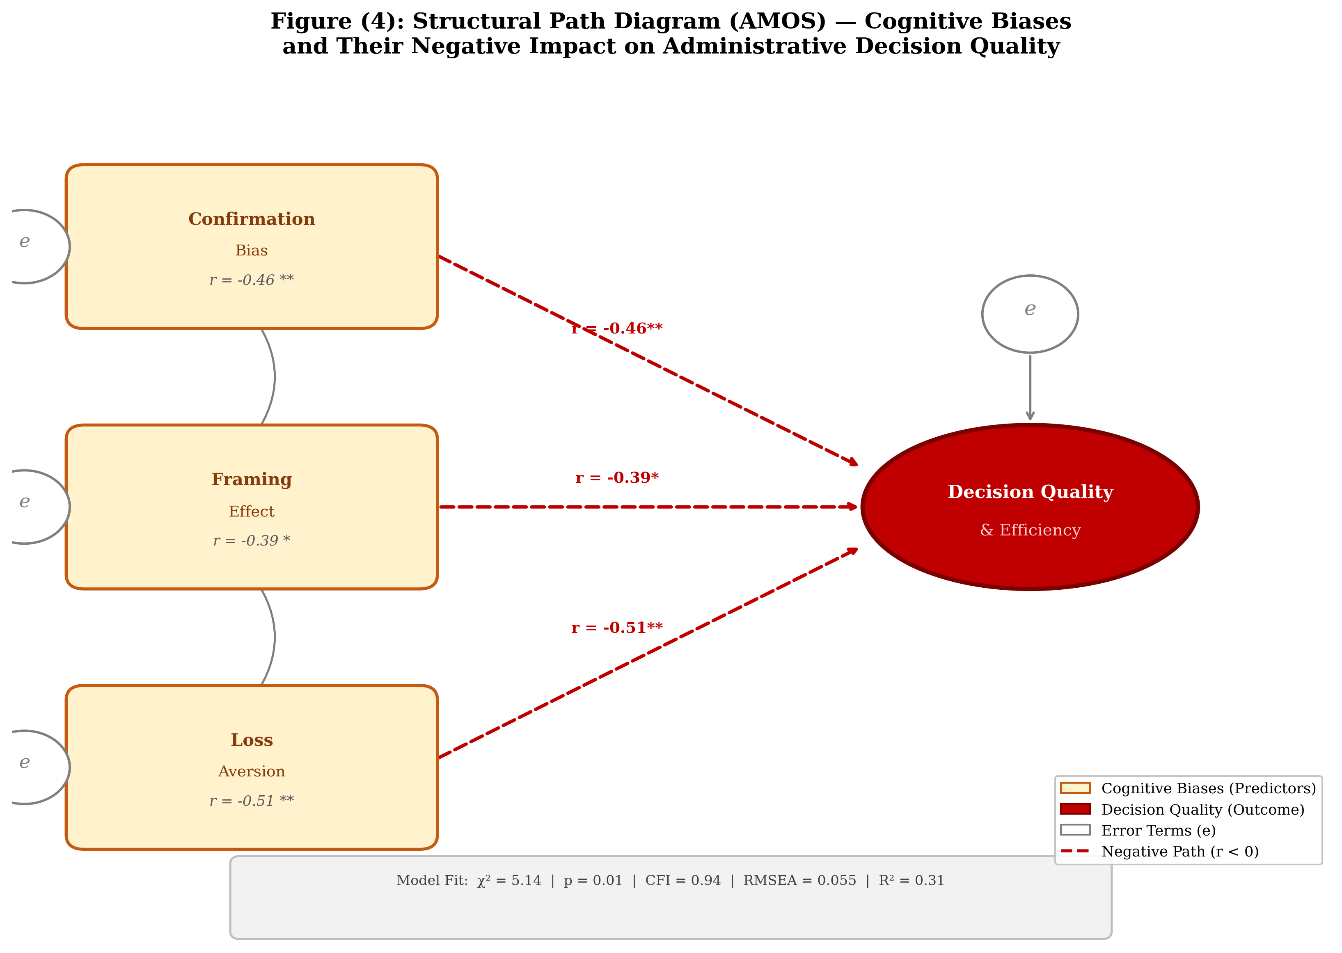
\includegraphics[width=\linewidth,keepaspectratio]{media/image9.png}
\else
  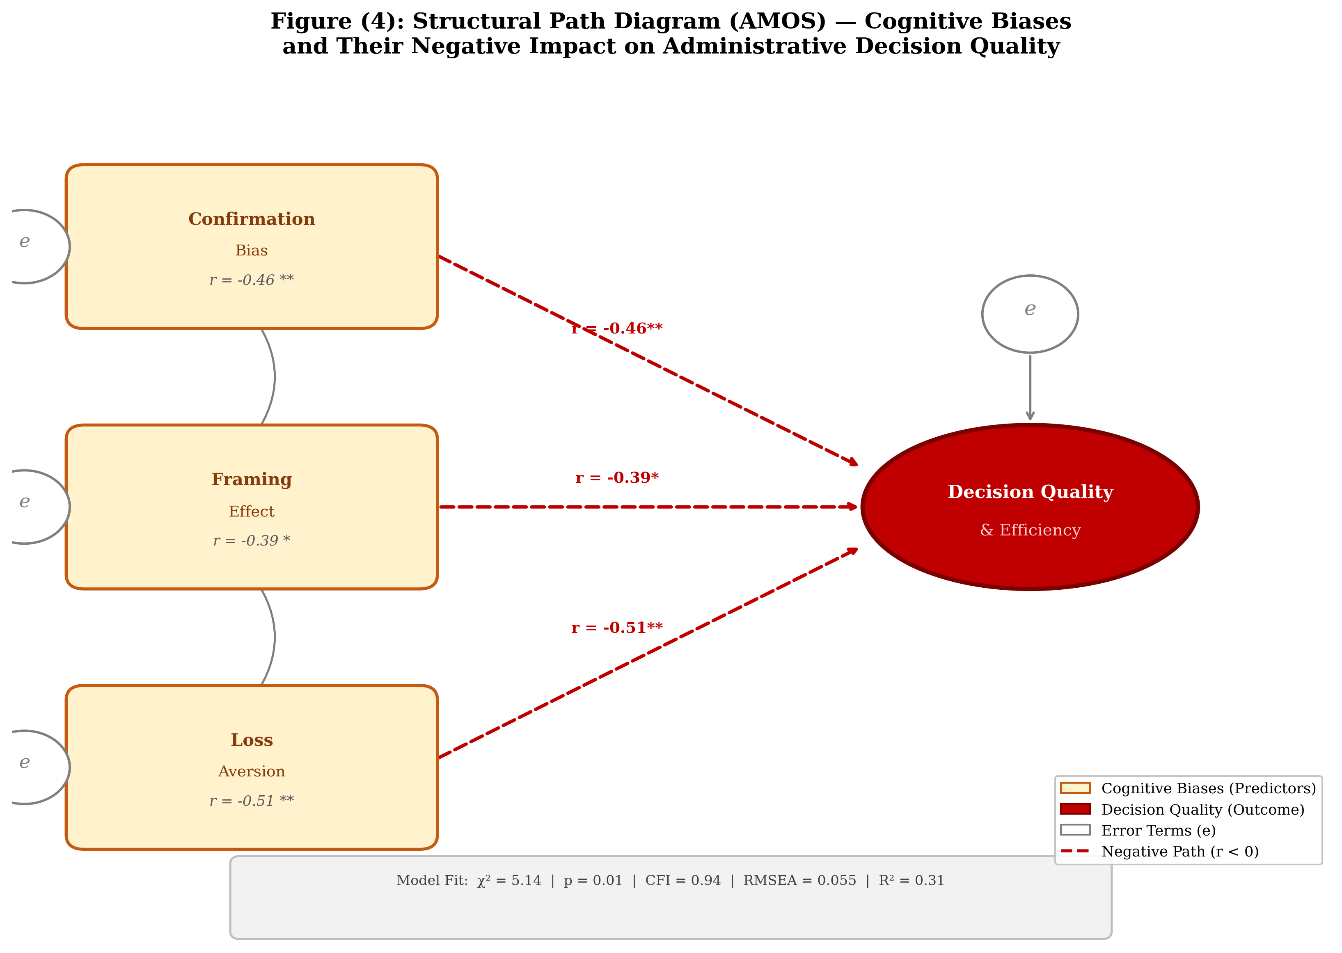
\includegraphics[width=5.3125in,height=3.7708in]{media/image9.png}
\fi
\caption{Figure 4}
\end{figure}\JLTXbelowplacement 

Figure (4) presents the structural equation model (AMOS) depicting the negative causal paths from three cognitive biases to administrative decision quality. Dashed arrows represent negative directional paths, consistent with the Spearman correlations reported in Table (2). The model fit indices (chi-squared = 5.14, CFI = 0.94, RMSEA = 0.055, R-squared = 0.31) indicate that the three biases collectively explain 31\% of the variance in decision quality. Covariance arrows between bias predictors reflect their inter-relatedness within the cognitive system. The researcher concludes that awareness of these biases — particularly loss aversion — is essential for improving the objectivity and effectiveness of educational administrative decisions.

Table (2) shows a statistically significant negative correlation between all the studied cognitive biases and the quality and efficiency of administrative decisions. Loss aversion recorded the highest negative correlation value (-0.51), indicating a relatively strong effect of this bias in weakening decision quality.

Confirmation bias came in second with a moderate negative correlation value (-0.46), reflecting leaders' tendency to reinforce their preconceived notions at the expense of objective alternatives. Framing bias recorded the lowest correlation value (-0.39), and although it had the least effect compared to the other biases, it remained statistically significant.

The researcher attributes this to the fact that cognitive biases function as mental shortcuts that reduce cognitive effort. However, in the educational administrative context, they lead to a narrowing of the range of alternatives and prioritizing institutional security over efficiency, especially within a culture of strict accountability that makes leaders more fearful of loss than of pursuing developmental gains.

3. Results of the third question: To what extent does the thinking style affect the effectiveness of administrative decisions among educational leaders? A paired samples t-test was used to compare the average effectiveness of managerial decisions when using rapid thinking versus analytical thinking, since the same participants evaluated both styles.

\JLTXaboveplacement \begin{jltxspan}%
\noindent\begin{minipage}{\linewidth}%
\centering
{\small
\begin{tabular}{|>{\centering\arraybackslash}p{\dimexpr 0.2221\linewidth-2\tabcolsep-\arrayrulewidth\relax}|>{\centering\arraybackslash}p{\dimexpr 0.2039\linewidth-2\tabcolsep-\arrayrulewidth\relax}|>{\centering\arraybackslash}p{\dimexpr 0.2123\linewidth-2\tabcolsep-\arrayrulewidth\relax}|>{\centering\arraybackslash}p{\dimexpr 0.1297\linewidth-2\tabcolsep-\arrayrulewidth\relax}|>{\centering\arraybackslash}p{\dimexpr 0.2281\linewidth-2\tabcolsep-\arrayrulewidth\relax}|}
\hline
\textbf{Thinking style} & \textbf{Arithmetic mean} & \textbf{Standard deviation} & \textbf{t-value} & \textbf{Significance level} \\
\hline
\cellcolor[HTML]{F2F2F2}\textbf{Fast thinking} & \cellcolor[HTML]{F2F2F2}\textbf{3.76} & \cellcolor[HTML]{F2F2F2}\textbf{0.71} & \cellcolor[HTML]{F2F2F2} & \cellcolor[HTML]{F2F2F2} \\
\hline
\textbf{Analytical thinking} & \textbf{4.48} & \textbf{0.52} & \textbf{4.21} & \textbf{0.001} \\
\hline
\end{tabular}}
\captionof{table}{Table 3: Results of the t-test on thinking styles and managerial decision effectiveness}%
\end{minipage}%
\end{jltxspan}\JLTXbelowplacement 

\JLTXaboveplacement \begin{figure}[H]
\centering
\ifdim 5.9375in>\linewidth
  
\includegraphics[width=\linewidth,keepaspectratio]{media/image10.png}
\else
  
\includegraphics[width=5.9375in,height=3.0729in]{media/image10.png}
\fi
\caption{Figure 5}
\end{figure}\JLTXbelowplacement 

Figure (5) displays the mean effectiveness scores of administrative decisions under two thinking styles, with error bars representing one standard deviation. Analytical thinking (M = 4.48, SD = 0.52) significantly outperformed fast thinking (M = 3.76, SD = 0.71), as confirmed by the paired-samples t-test result (t(29) = 4.21, p \textless{} .001, shown in the significance bracket). The red dashed reference line at the scale midpoint (4.0) highlights that analytical thinking exceeds this threshold while fast thinking falls below it in terms of decision effectiveness. The researcher attributes this superiority to the capacity of analytical thinking for deeper information processing, more thorough evaluation of alternatives, and better consideration of long-term consequences — all critical competencies in the complex human and organizational context of educational institutions.

\JLTXaboveplacement \begin{figure}[H]
\centering
\ifdim 5.7604in>\linewidth
  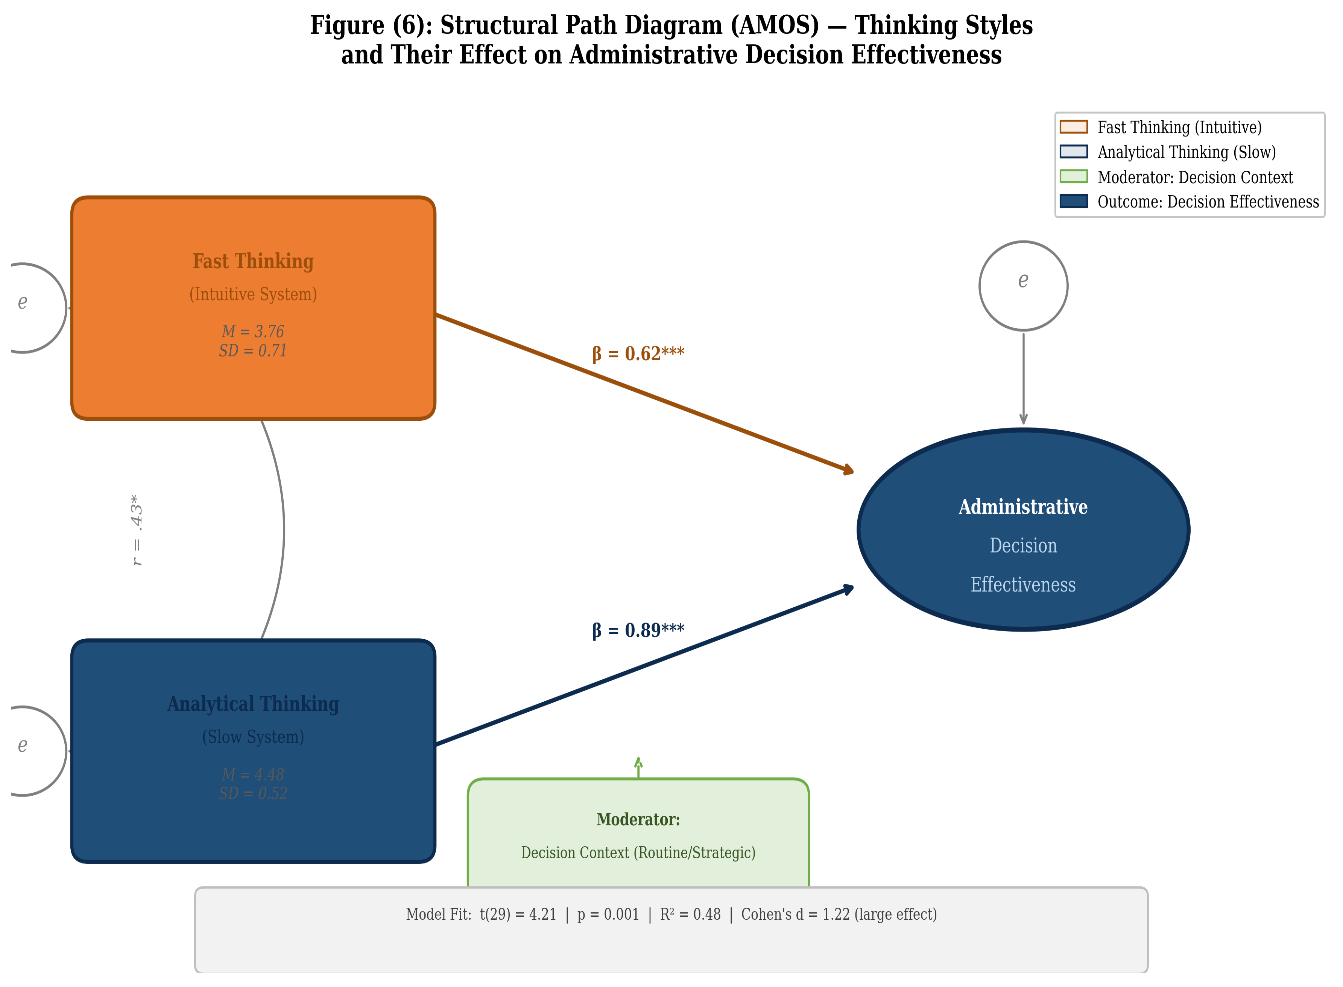
\includegraphics[width=\linewidth,keepaspectratio]{media/image11.png}
\else
  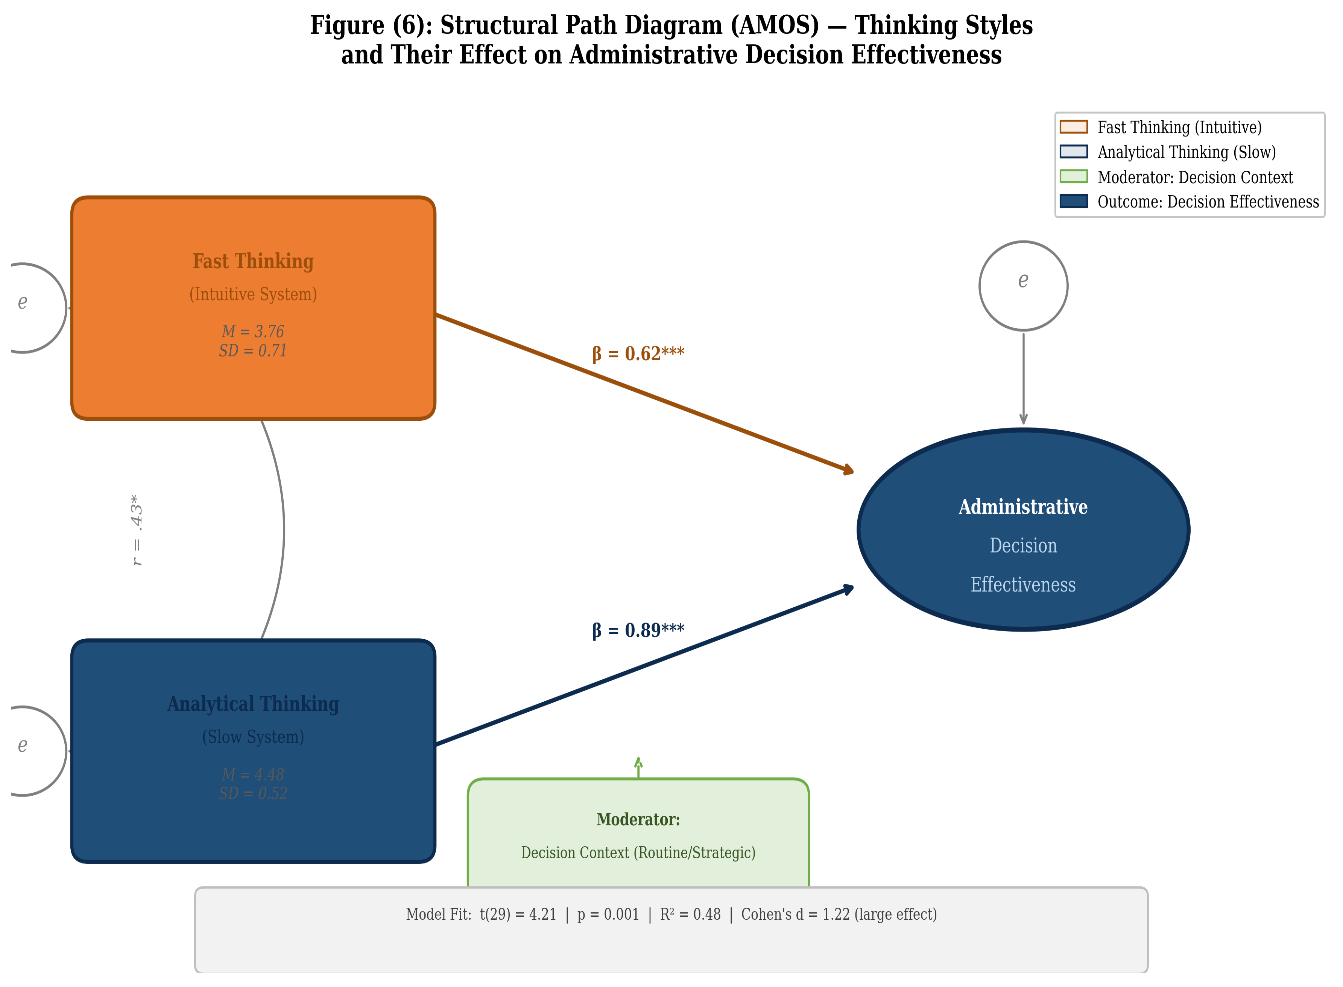
\includegraphics[width=5.7604in,height=3.8958in]{media/image11.png}
\fi
\caption{Figure 6}
\end{figure}\JLTXbelowplacement 

Figure (6) presents the structural path diagram (AMOS) modeling the differential effects of thinking styles on administrative decision effectiveness. Analytical thinking exerted a substantially stronger positive path (beta = 0.89***) compared to fast thinking (beta = 0.62***), with the outcome variable (decision effectiveness) achieving an explained variance of R-squared = 0.48. A moderator variable (decision context: routine vs. strategic) is incorporated into the model, reflecting the theoretical understanding that context determines which thinking style is most appropriate. The bidirectional covariance arrow between the two thinking styles (r = .43*) indicates that they are not mutually exclusive but complementary cognitive capacities. The researcher recommends designing leadership training programs that develop leaders' ability to consciously switch between thinking styles according to the nature and urgency of each administrative situation.

Table (3) shows statistically significant differences in the average effectiveness of administrative decisions based on the thinking style used. Analytical thinking achieved a significantly higher average (4.48) compared to rapid thinking (3.76), and the high value of the t-test indicates the strength of this difference.

The researcher attributes this superiority to the fact that analytical thinking allows for deeper processing of information, weighing of alternatives, and consideration of the long-term effects of the decision. This is crucial in the educational environment, which is characterized by the interplay of human and organizational factors. In contrast, rapid thinking remains less effective when dealing with critical or complex decisions.

Fifth: Results and Discussion:

\begin{itemize}
  \item The study results showed that cognitive psychological factors play a pivotal role in the administrative decision-making process of educational leaders. Analytical and systematic thinking was found to be the most prominent factor compared to others, reflecting leaders' awareness of the importance of analysis and deliberation in complex administrative situations.
  \item The results revealed a significant prevalence of rapid, intuitive thinking among educational leaders, especially in urgent or unclear situations. This aligns with what psychological literature indicates about individuals resorting to rapid thinking under time pressure and incomplete information.
  \item The study demonstrated a statistically significant negative correlation between confirmation bias and the quality of administrative decisions. This suggests that a leader's reliance on information that confirms their pre-existing beliefs reduces the objectivity of the decision and weakens its outcomes.
  \item The results showed that cognitive framing clearly influences the choices of educational leaders. Their responses change depending on how information is presented, whether positively or negatively, a finding supported by cognitive psychology theories. 5. The study revealed that a low tolerance for ambiguity among some educational leaders is linked to increased hesitation and excessive caution in decision-making, which may limit their ability to make bold decisions in unstable situations.
  \item Statistical comparisons showed statistically significant differences in the effectiveness of administrative decisions attributable to thinking style. Analytical thinking outperformed rapid thinking in achieving more accurate and sustainable decisions.
  \item The results indicated that the quality of administrative decisions is positively correlated with the use of data and systematic information analysis, which enhances decision reliability and reduces the likelihood of error, the study pointed out that time pressures and broad administrative responsibilities contribute to an increased reliance on rapid thinking, which raises the likelihood of cognitive biases.
  \item The study's findings clearly align with educational literature, which emphasizes that collective and participatory decision-making reduces the impact of individual biases and improves the quality of administrative decisions. 10. The study concluded that integrating the cognitive psychology perspective into administrative decision analysis provides a deep explanatory framework for understanding the behavior of educational leaders, and contributes to developing more effective models for decision-making in educational institutions.
\end{itemize}

Sixth: Recommendations:

\begin{itemize}
  \item The necessity of incorporating cognitive psychology concepts into educational leadership development and training programs, given their role in enhancing awareness of thinking patterns and cognitive biases, and Designing specialized training programs to develop analytical thinking skills and data-driven decision-making within educational institutions.
  \item Promoting a culture of deliberation and systematic thinking in strategic administrative decisions, especially those with long-term implications, Creating supportive educational work environments that reduce psychological and time pressures, thereby contributing to improved quality of administrative decisions.
  \item Encouraging participatory decision-making methods and involving work teams in analyzing alternatives and formulating solutions, Developing self-diagnostic tools to help educational leaders discover their prevailing thinking patterns and identify strengths and weaknesses in their administrative practices.
  \item Udies examining the impact of demographic variables and professional experience on the relationship between cognitive psychology factors and administrative decision-making, Integrate the findings of contemporary psychological research into the development of educational policies to ensure more realistic and effective decision-making.
  \item Establish advisory support units within educational institutions to assist leaders in complex decisions with psychological and organizational dimensions.
\end{itemize}

Data Availability

The datasets used and/or analyzed during the current study are available from the corresponding author on reasonable request.

Competing Interests

The author declares that there are no competing interests.

Funding

No funding was received for this research.

References:

[1] Rikabi, A. (2018). Educational and Administrative Decision-Making: Between Reality and Aspiration. Amjad Publishing and Distribution House.

[2] Khashab, D. (2022). Role Models in Education. Journal of Sustainable Studies, 4, ( 4), pp. 2498-2520.

[3] Hindawi, S. (2020). The Role of Servant Leadership in Achieving Institutional Excellence: An Applied Study on Non-Governmental Hospitals in the Gaza Strip. Unpublished Master's Thesis, Islamic University of Gaza.

[4] Alrashdan, H; Darawsheh, N; Aabed, S; Bsoul, M; Ganayem, S; and Mhameed, M. (2023). Analyzing University Administration's Impact on Faculty Digital Self-Learning, Journal of Statistics Applications and Probability, 12, 1591–1601

[5] Jarim, A. (2021). Psychology and its Impact on Education. Arab Press Agency.

[6] ALAwAmRAh, A , Ajmi, H, Darawsheh, N , Darawsheh, O, Urabi, O.(2024).Analyzing Student's Perceptions about the Values of Digital Citizenship, Journal of Statistics Applications and Probability, 2024, 13(4), pp. 1279–1288.

[7] Brabah, A. (2019). Decision-Making in the Organization and its Relationship to Management Information Systems, Journal of Economic Studies, Vol. 13, No. 3, pp. 226-249.

[8] Hatamala, H ,Darawsheh, N. (2019). The Challenges of the Application of the Productive University’s Philosophy In Jordanian Universities and Ways of Developing Them from The Perspective of Academic Leaders, Journal of Institutional Research South East Asia, 17(1), pp. 93–117,(2019).

[9] Batayneh, A. (2017). The Efficiency of Public Secondary School Principals in Wadi Al-Seer District in Involving Teachers in the Decision-Making Process and its Relationship to their Job Performance from the Teachers' Perspective (Unpublished Master's Thesis). University of Jerash, Jerash.

[10] Darawsheh, N. (2018). The Reality of The Challenges Faced By Graduate Students In The Faculties Of Educational Sciences In Jordanian Universities, JIRSEA, 16(2),132-140,(2018).

[11] Alkharman , J ,. Drawsheh ,. S,. Al-Khataybeh , M,. BaniYounes , Z,. Darawsheh , N,. Alrashdan, H,. (2024). Cyber Attacks and its Implication to National Security: The Need for International Law Enforcement, Pakistan Journal of Criminology, 16(3), pp. 851–864

[12] Belhaj, F. (2016). The Theoretical and Scientific Foundations of Decision-Making. Algerian Journal of Globalization and Economic Policies, No. 7, pp. 269-284.

[13] Taqi, A. (2019). The Relationship between Strategic Planning and Organizational Performance: A Field Study, Journal of Economics and Human Development, 10 (1), pp. 131-153.

[14] Hattab, S. (2020). The Role of the Administrative Apparatus in Public Decision-Making in Morocco, Journal of Law and Business, 16, pp. 127-155.

[15] Yassin Al-Sheikh, K. (2011). Thinking Patterns. University of Damascus, Syria.

[16] Sanawi, F., \& Hamel, M. (2020). Creative Thinking and its Relationship to Academic Achievement: A Descriptive Study of Third-Year Intermediate School Students in the Wilaya of Relizane. Journal of Social Sciences, 14(2), pp. 147-157.

[17] Alrashdan, H., Darawsheh, N., Almheiri, A., Aljanabi, Y., Al-Khataybeh, M., \& Al-Quran, N. (2025). The Effect of Administrative Bullying on the Quality of Education. Educational Process: International Journal, 18, e2025515.

[18] Sukhni, A. (2019). Strategic Thinking and its Impact on the Performance of Jordanian Private Universities (Unpublished Master's Thesis). Al al-Bayt University, Mafraq.

[19] Darawsheh, N; Al-Khataybeh, M; Alrashdan, H; Drawsheh, S; Abu Grarh, A; and abu dogush, M .(2024) "Coexistence skills among mothers of children with multiple disabilities in the northern region of Jordan (IRBID), Journal of Statistics Applications \& Probability: 13( 2), 665-680.

[20] Rashwan, A. (2018). The Impact of Burnout on the Performance Level of Accountants Working for the Palestinian Ministry of Finance in the Gaza Strip. Journal of Research in Financial and Accounting Sciences, No. 6, pp. 31-56.

[21] Darawsheh, N , Alrashdan, H , Al-Khataybeh, M , Al Ajmi, H , almheiri, A , Shaglof,A , Aldarmaki, I , BaniYounes, Z and Aidi,R .(2025). The Degree of Impact of Organizational Intelligence Obstacles in the Digital Age, Journal of Statistics Applications \& Probability, An International Journal, 14(6), 985-995.

[22] Salem, S. (2020). Forecasting and Decision-Making Methods: The Epidemiological Modeling Tool, International Politics Journal, Vol. 55, Supplement, pp. 25-28.

[23] Rabee, W. (2022). The Importance of Think Tanks and Strategic Studies in Decision-Making. International Politics Journal, 57, ( 228), pp. 296-301.

[24] Mabrouk, M. (2021). Emotional Intelligence as a Predictor of Successful Leadership. The Educational Journal, Issue 18, pp. 423-448

[25] Balata, N. (2021). The Impact of Organizational Health on Strategic Performance: An Application to the Palestinian Red Crescent Society in the Gaza Strip (Unpublished Master's Thesis), Islamic University (Gaza), Gaza.

[26] Midtgård . K and Selart, M. (2025). Cognitive biases in strategic decision-making, Administrative Sciences, 15(6), 227 (2025). https://doi.org/10.3390/admsci15060227

[27] Hamoud, A. (2022). Strategic Alignment and its Reflection in Enhancing Entrepreneurial Performance. Al-Ghari Journal of Economic and Administrative Sciences, Vol. 18, No. 2, pp. 789-810.

[28] Abdo, M., Jumaa, B., Al-Amin, A., Al-Rifai, M., and Al-Rifai, D. (2023). Critical Thinking and its Impact on Enhancing Intellectual Security: A Theoretical and Field Study. Journal of Arts, Literature, Humanities and Social Sciences, No. 92, pp. 1-34.

[30] Darawsheh, N, Alrashdan, H, Alzawaideh, M, Thaer Ajouly, Almheiri, A, Aldarmaki, I .(2024). Administrative Empowerment Among Academic Leaders And its Relationship to the Quality of Work Life of Faculty Member, Journal of Ecohumanism, 3(7), 5172–5184

[31] Darafli, A. (2020). Education in Light of Psychological Studies. Arab Press Agency

[32] Hamad, F. (2019). The Impact of Knowledge Management Processes on the Quality of Decision-Making: A Field Study on Jordanian Pharmaceutical Companies (Unpublished Master's Thesis). Al-Isra Private University, Amman

\end{document}
